\section{Evaluation}
\label{es:sec:evaluation}

\subsection{Methodology}
\label{es:sec:methodology}

% \subsection{Experimental Setup}
% \label{es:subsec:expsetup}

The benchmarks were executed on an Intel Xeon E3-1275 v6 with 4 HT cores clocked at 3.8 GHz with 64 GB of RAM and SSD drives running Fedora 37. We disabled frequency scaling, turbo boost and swap space during the experiments.
% <<<<<<< Updated upstream
% %but left HT enabled.
% =======
% >>>>>>> Stashed changes

We are using a two-process configuration, depicted in \Cref{es:fig:func-setup}. For every client request, 
%On every request received from the client to the producer process, 
the producer process sends $n$ requests of $m$ KB to the consumer process. We evaluate values of 1, 10 and 20 for $n$ and, where possible, values from $2^{0}$ to $2^{9}$ for $m$. CoFaaS only optimizes the inter-function communication latency, i.e., the latency occurring when the producer process in \Cref{es:fig:func-setup} calls the consumer process.
% The latency incurred when the client calls the producer process is not targeted by the CoFaaS transformation.
Therefore, adjusting the value of $n$ (request repetitions) allows us to estimate the performance impact of CoFaaS on larger applications that perform a variable number of inter-function requests. We refer to requests occurring within the application as \emph{inter-function} requests. The benchmarked  application and invocation client were adapted from \cite{ustiugov:benchmarking}.

We evaluate two functionally equivalent implementations of the application shown in \Cref{es:fig:func-setup} written in the languages Go~\cite{golang} and Rust~\cite{rust}, respectively. The key distinction between the two languages is that Go uses a Garbage Collector (GC) for memory management whereas Rust inserts compile-time instructions to handle memory. Go therefore relies on a managed runtime for execution. Since languages using managed runtimes have different performance characteristics and platform requirements than unmanaged languages, our experiments demonstrate that the CoFaaS is %functional and 
effective in both cases.

Compilers, with Wasm targets
%suitable for use outside of a 
other than
web browsers, need to support the WebAssembly System Interface (WASI). For Rust, Wasm support is generally good and its compiler supports a usable WASI target. However, the WASI target of the mainline Go compiler is currently not supported by the Wasm component model. Instead, we are limited to using the TinyGo compiler which primarily targets small embedded devices. For this reason, it is positioned at a different design point than a compiler targeting general-purpose systems. In particular, its garbage collector implementation is optimized for code size rather than speed causing its GC performance to trail the mainline Go compiler \cite{tinygo_gc}. Because of this, our example application implemented in Go is heavily penalized when executed on Wasm. Therefore, we disable GC for our Go benchmarks. Naturally, this limits how long we can run our benchmarks for and the payload sizes we can use. When running on Wasm, we are further limited by the current Wasm specification only supporting 32-bit pointers~\cite{rossberg22_webas_core_specif}. In our case, this means that we can only evaluate our Go application with a payload size of up to 16KB, as the experiment otherwise runs out of memory. These limitations are unrelated to CoFaaS, and, at the time of writing, efforts are underway to alleviate both of these limitations~\cite{bindgen-todo,wasm64}. 

For the round-trip-time benchmarks (\Cref{es:subsec:rtt}), we invoke 6,000 requests back-to-back for every configuration. We chose this number of requests to get a representative number of data points while not exceeding memory capacity in the non-GC configurations. For evaluating the latency of inter-function requests, we report the mean of 100 inter-function requests and we repeat each experiment 100 times.

\begin{figure}
  \centering
  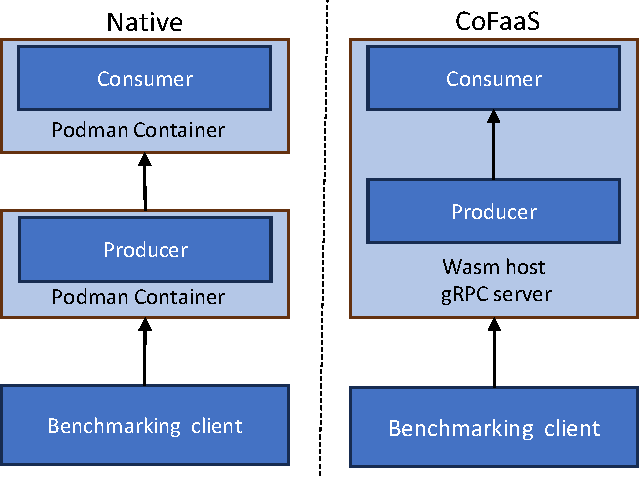
\includegraphics[width=0.6\columnwidth]{figures/setup}
  \caption{\label{es:fig:deploy-setup} The deployment configurations for the native and the CoFaaS benchmarks.}
\end{figure}

To mimic a common real-world deployment scenario, each native function is deployed in a separate Podman container. The CoFaaS benchmarks are run inside a Wasm host written in Rust that embeds the Wasmtime~\cite{wasmtime} runtime. This host loads the CoFaaS component and externally exposes the gRPC interface of the Producer function (using the Tonic gRPC library). When the host receives an external gRPC request, it translates and proxies the request to the CoFaaS application. This experiential setup is depicted in \Cref{es:fig:deploy-setup}.
Finally, we point out that we run our native FaaS application on the same machine without any other functions running at the same time. We consider this a highly optimized baseline compared to, for example, deploying our functions to a public cloud. The speedups achieved by CoFaaS could therefore increase further if a more realistic baseline was used.

% \truls{Mention that we run the two functions on the same machine and therefore we use a highly optimized baseline}


\subsection{Round-trip Latency}
\label{es:subsec:rtt}

\begin{figure}
  \centering
  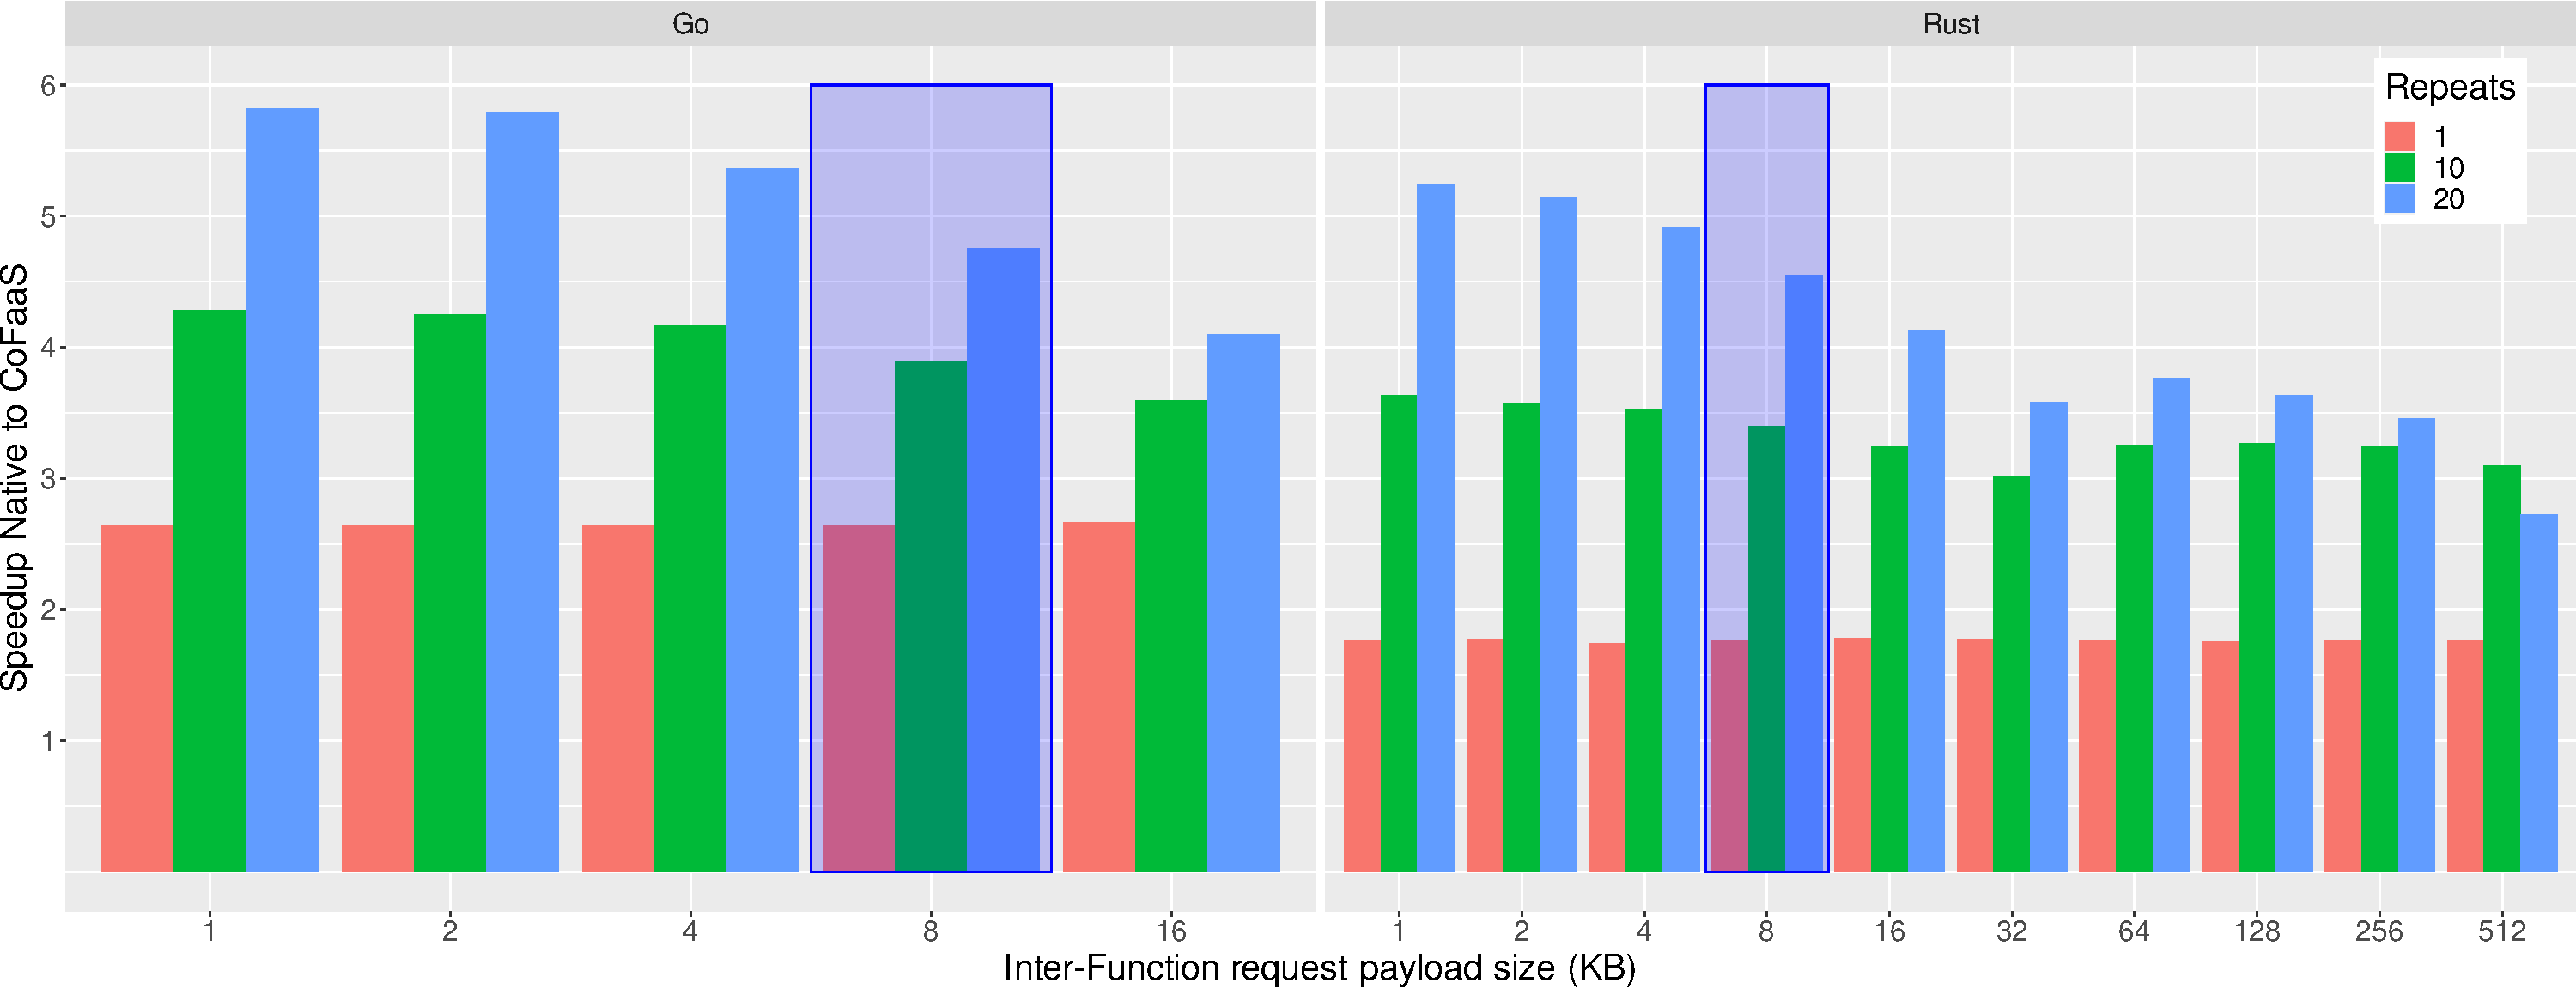
\includegraphics[width=\textwidth]{figures/rust-go}
  \caption{\label{es:fig:rtt-latency} The round-trip latency of issuing a request to our example application.}
\end{figure}

We begin our evaluation of CoFaaS' performance by showing measurements of the request round-trip latency. The round-trip latency is defined by the time it takes before the requesting client receives the reply to a request that it sent. The speedups achieved by the CoFaaS optimized application over the native baseline are shown in \Cref{es:fig:rtt-latency}. The blue boxes mark the median request payload size as observed from traces of real-world FaaS deployments on the Azure cloud \cite{mahgoub22_wisef} and is hence a notable data point. We run the Rust benchmarks with payload sizes between 1 and 512 whereas the Go benchmarks are run for sizes between 1 and 16. Due to the GC limitations outlined in \Cref{es:sec:methodology}, we are unable to run the Go benchmark for the full range of payload sizes. In both cases, we perform 1, 10 and 20 inter-function calls per external request.

\Cref{es:fig:rtt-latency} shows that the payload size does not impact configurations that issue only a single inter-function call, i.e., CoFaaS consistently yields speedups of 2.75$\times$ and 1.75$\times$ for Go and Rust, respectively. The reason is that a single inter-function call accounts for a moderate but significant fraction of the complete request round-trip time. Thus, as we increase the number of inter-function calls, the achieved speedup also increases. Peak speedups are achieved when an inter-function 1KB request is repeated 20 times, yielding a $5.9\times$ speedup for Go and $5.2\times$ for Rust. This shows that the beneficial impact of CoFaaS is larger for applications that perform a lot of inter-function requests.

%However, even in the single call configuration speedups are significant yielding 2.75$\times$ and 1.75$\times$ for Go and Rust respectively.

% [Add plots showing raw latencies to explain why speedups are going down. The explanation is that for large payload sizes the cost of moving data becomes dominating regardless of how we do it. Argue that large requests are out of scope]


A general trend is that speedups increase with smaller payload sizes. The intuition behind this is that regardless of how we make the request, we need to copy data from the producer process to the consumer. The performance of this underlying memory copy operation is limited by the hardware and therefore limits the performacne opportunity available for CoFaaS. To support this observation, we provide the raw latency numbers in \Cref{es:fig:lat-numbers}. Here, we see that with increasing payload sizes, the time needed by the native invocation and CoFaaS converges. Since the objective of CoFaaS is to reduce the \emph{latency} of requests, rather than the transfer rate, dealing with such larger requests is outside the scope of CoFaaS.
% rakesh{I would put it differently and say that the opportunity is less because XXX.}.
Furthermore, as previously stated, an analysis of Azure FaaS traces showed that the median request payload size is a mere 8KB, well within the range where CoFaaS gives performance improvements. Further, to our knowledge, it is uncommon to move large amounts of data using RPC requests in FaaS applications. In such cases, using external storage to transfer data between the functions is preferred. Still, we emphasize that even if the relative speedups yielded by CoFaaS decrease with increasing request sizes, the absolute reduction in round-trip times is still significant. For example, for the 512KB payload size the round-trip-time decreases from 20ms to 7ms; a significant improvement with a potentially big impact on application responsiveness.

% \magnus{I'm not fully convinced by this argument. The latencies appear low in all cases. In relative terms, we still cut round trip time by more than half (20 ms to 7ms) -- and that is significant! So maybe we should simply say that speedups are lower but still significant. So then there is a question if we want to show Figure~\ref{es:fig:lat-numbers}.}

% \truls{What does ``very real'' mean in this context}

\begin{figure}
  \centering
  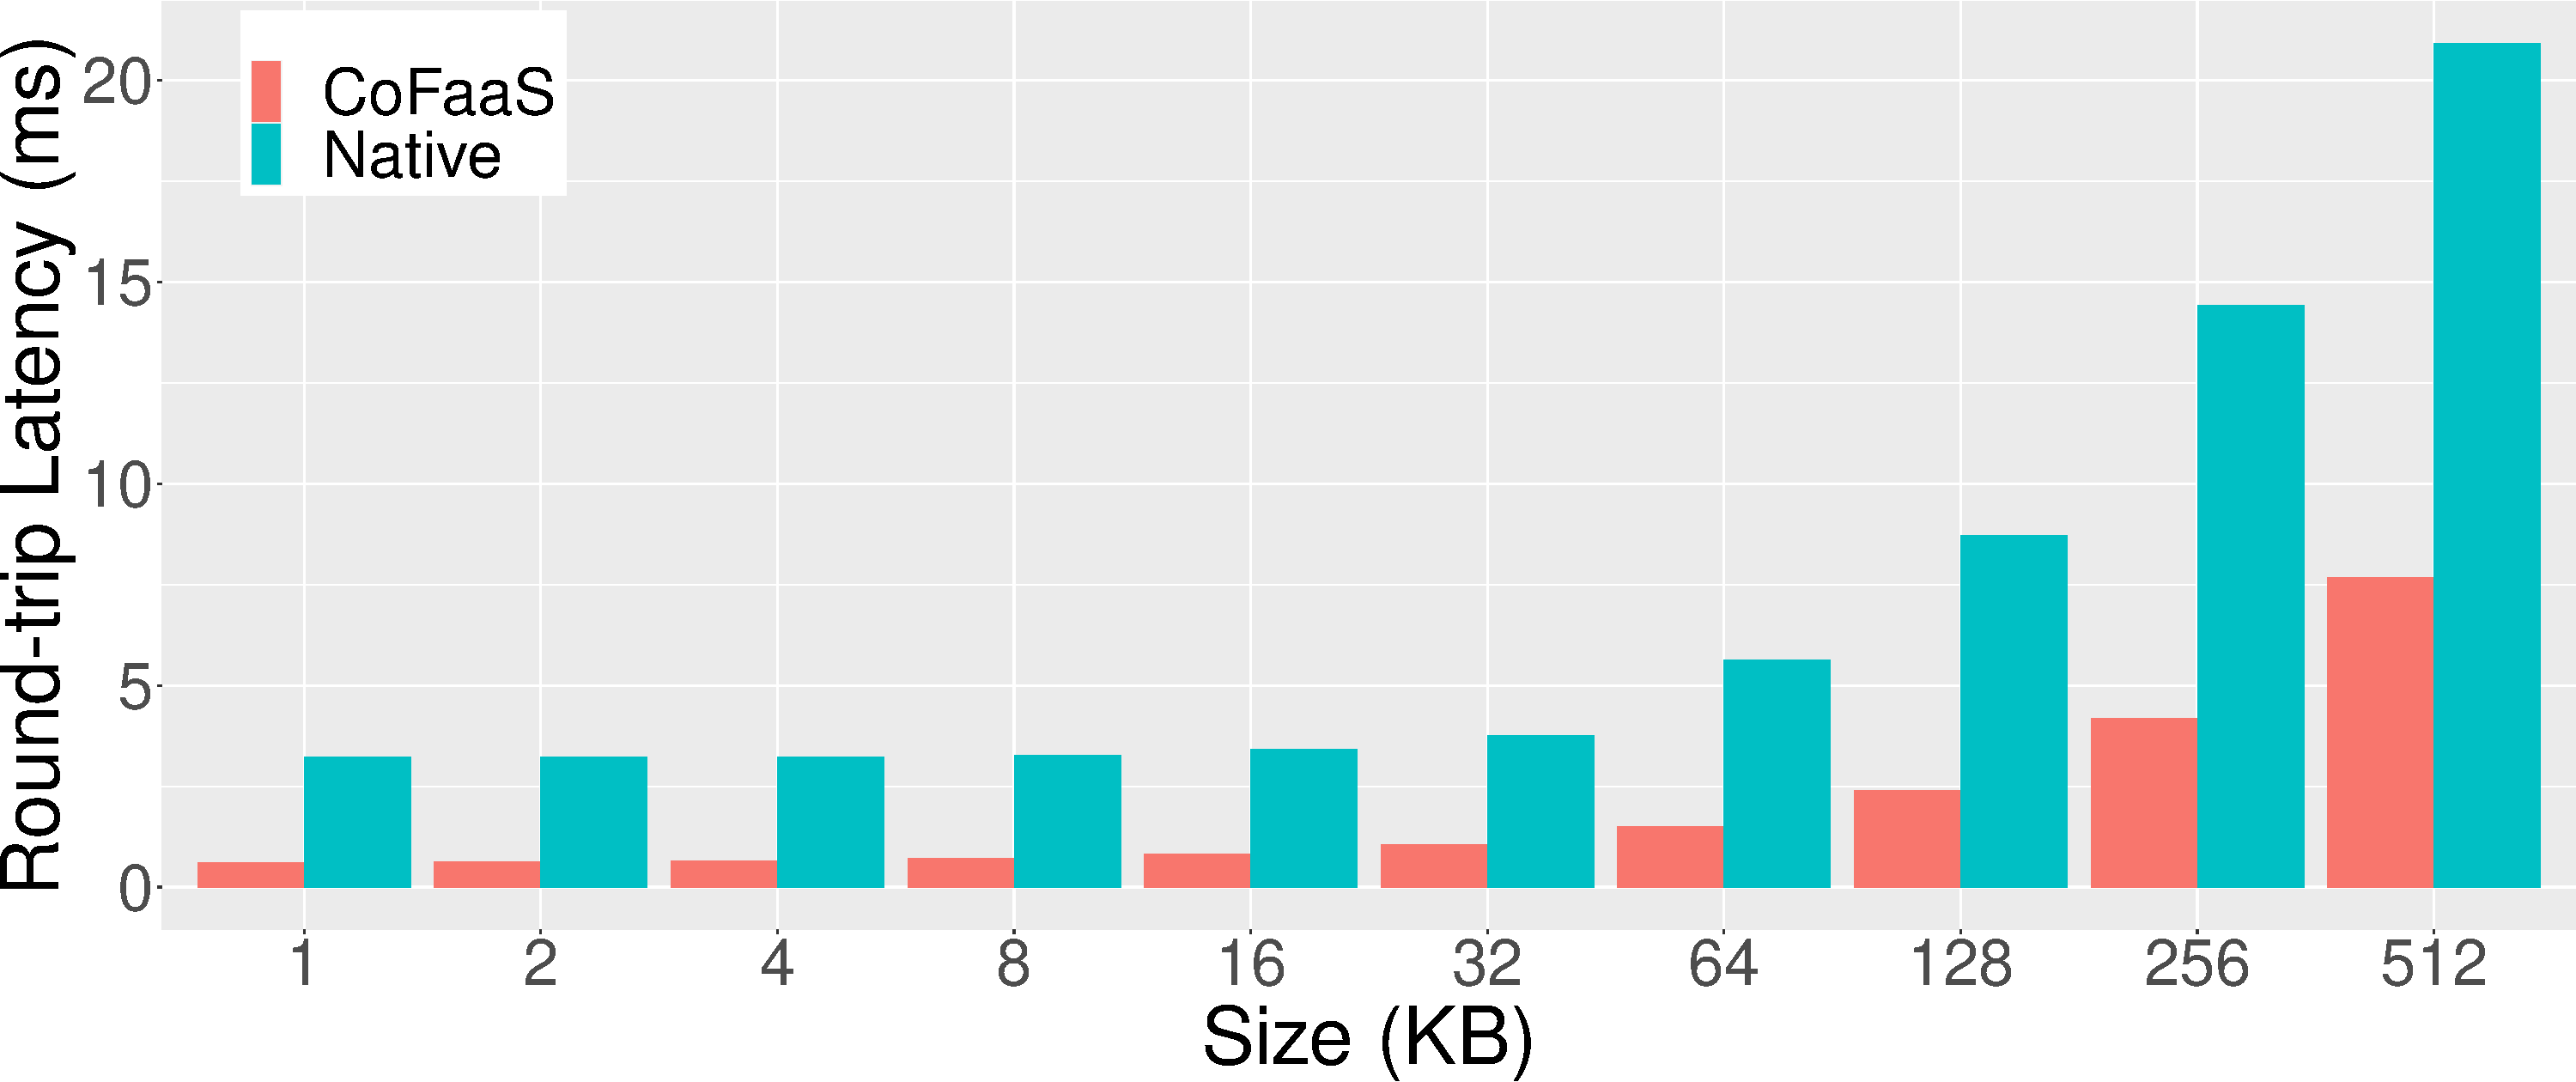
\includegraphics[width=\columnwidth]{figures/rawlat.pdf}
  \caption{\label{es:fig:lat-numbers} Latency (ms) of the Rust application performing 20 inter-function requests when running natively and using the CoFaaS transformation}
\end{figure}

% [Comment on the durability of the results, i.e. how speedups will increase significantly if we compare against running the native configuration where the two functions run on different machines]

\subsection{Inter-Function Request Latency}
\label{es:subsec:intra-app-latency}

\begin{figure}
  \centering
  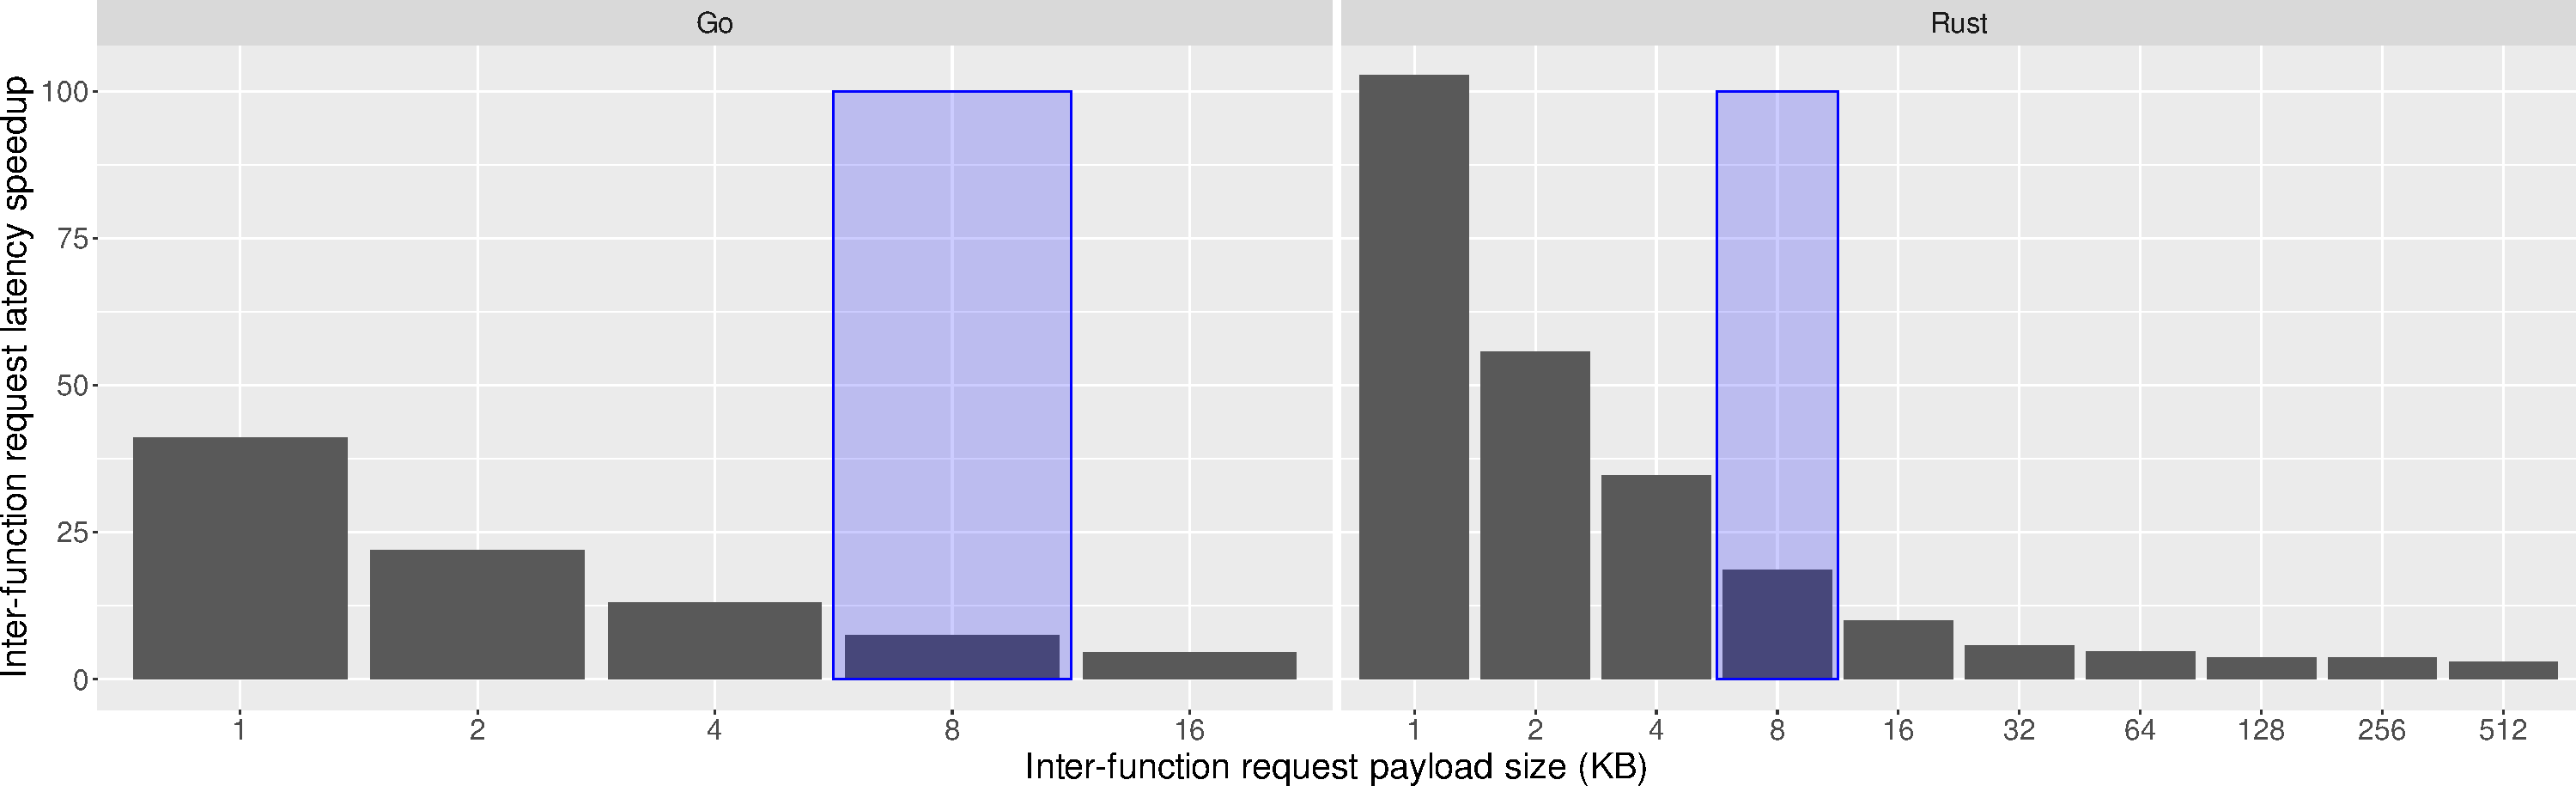
\includegraphics[width=\textwidth]{figures/rust-go-latency}
  \caption{\label{es:fig:req-latency} The speedups of a single request.}
\end{figure}

Next, we narrow the scope of our investigation to the latency of inter-function requests; the primary target of CoFaaS. \Cref{es:fig:req-latency} shows the speedups of the CoFaaS optimized application over the native baseline when measuring the latency of a single request. Compared to the results in \Cref{es:fig:rtt-latency}, the speedups are significantly higher as this measurement bypasses constant factors involved in every request issued to the application.

This result cements that CoFaaS is highly effective at reducing the latency of inter-function calls in serverless applications. For the Rust application with a 1KB request payload size, we see a $100\times$ speedup. Similar to our round-trip time evaluation, we see diminishing returns when increasing payload sizes. We can understand this trend using the same intuition as before; for larger payload sizes, the time needed to transfer the request payload data becomes dominating regardless of the transfer method used.


\subsection{Impact of Go Garbage Collection}
\label{es:subsec:sensitivity}

% \begin{figure}[ht]
%   \centering
%   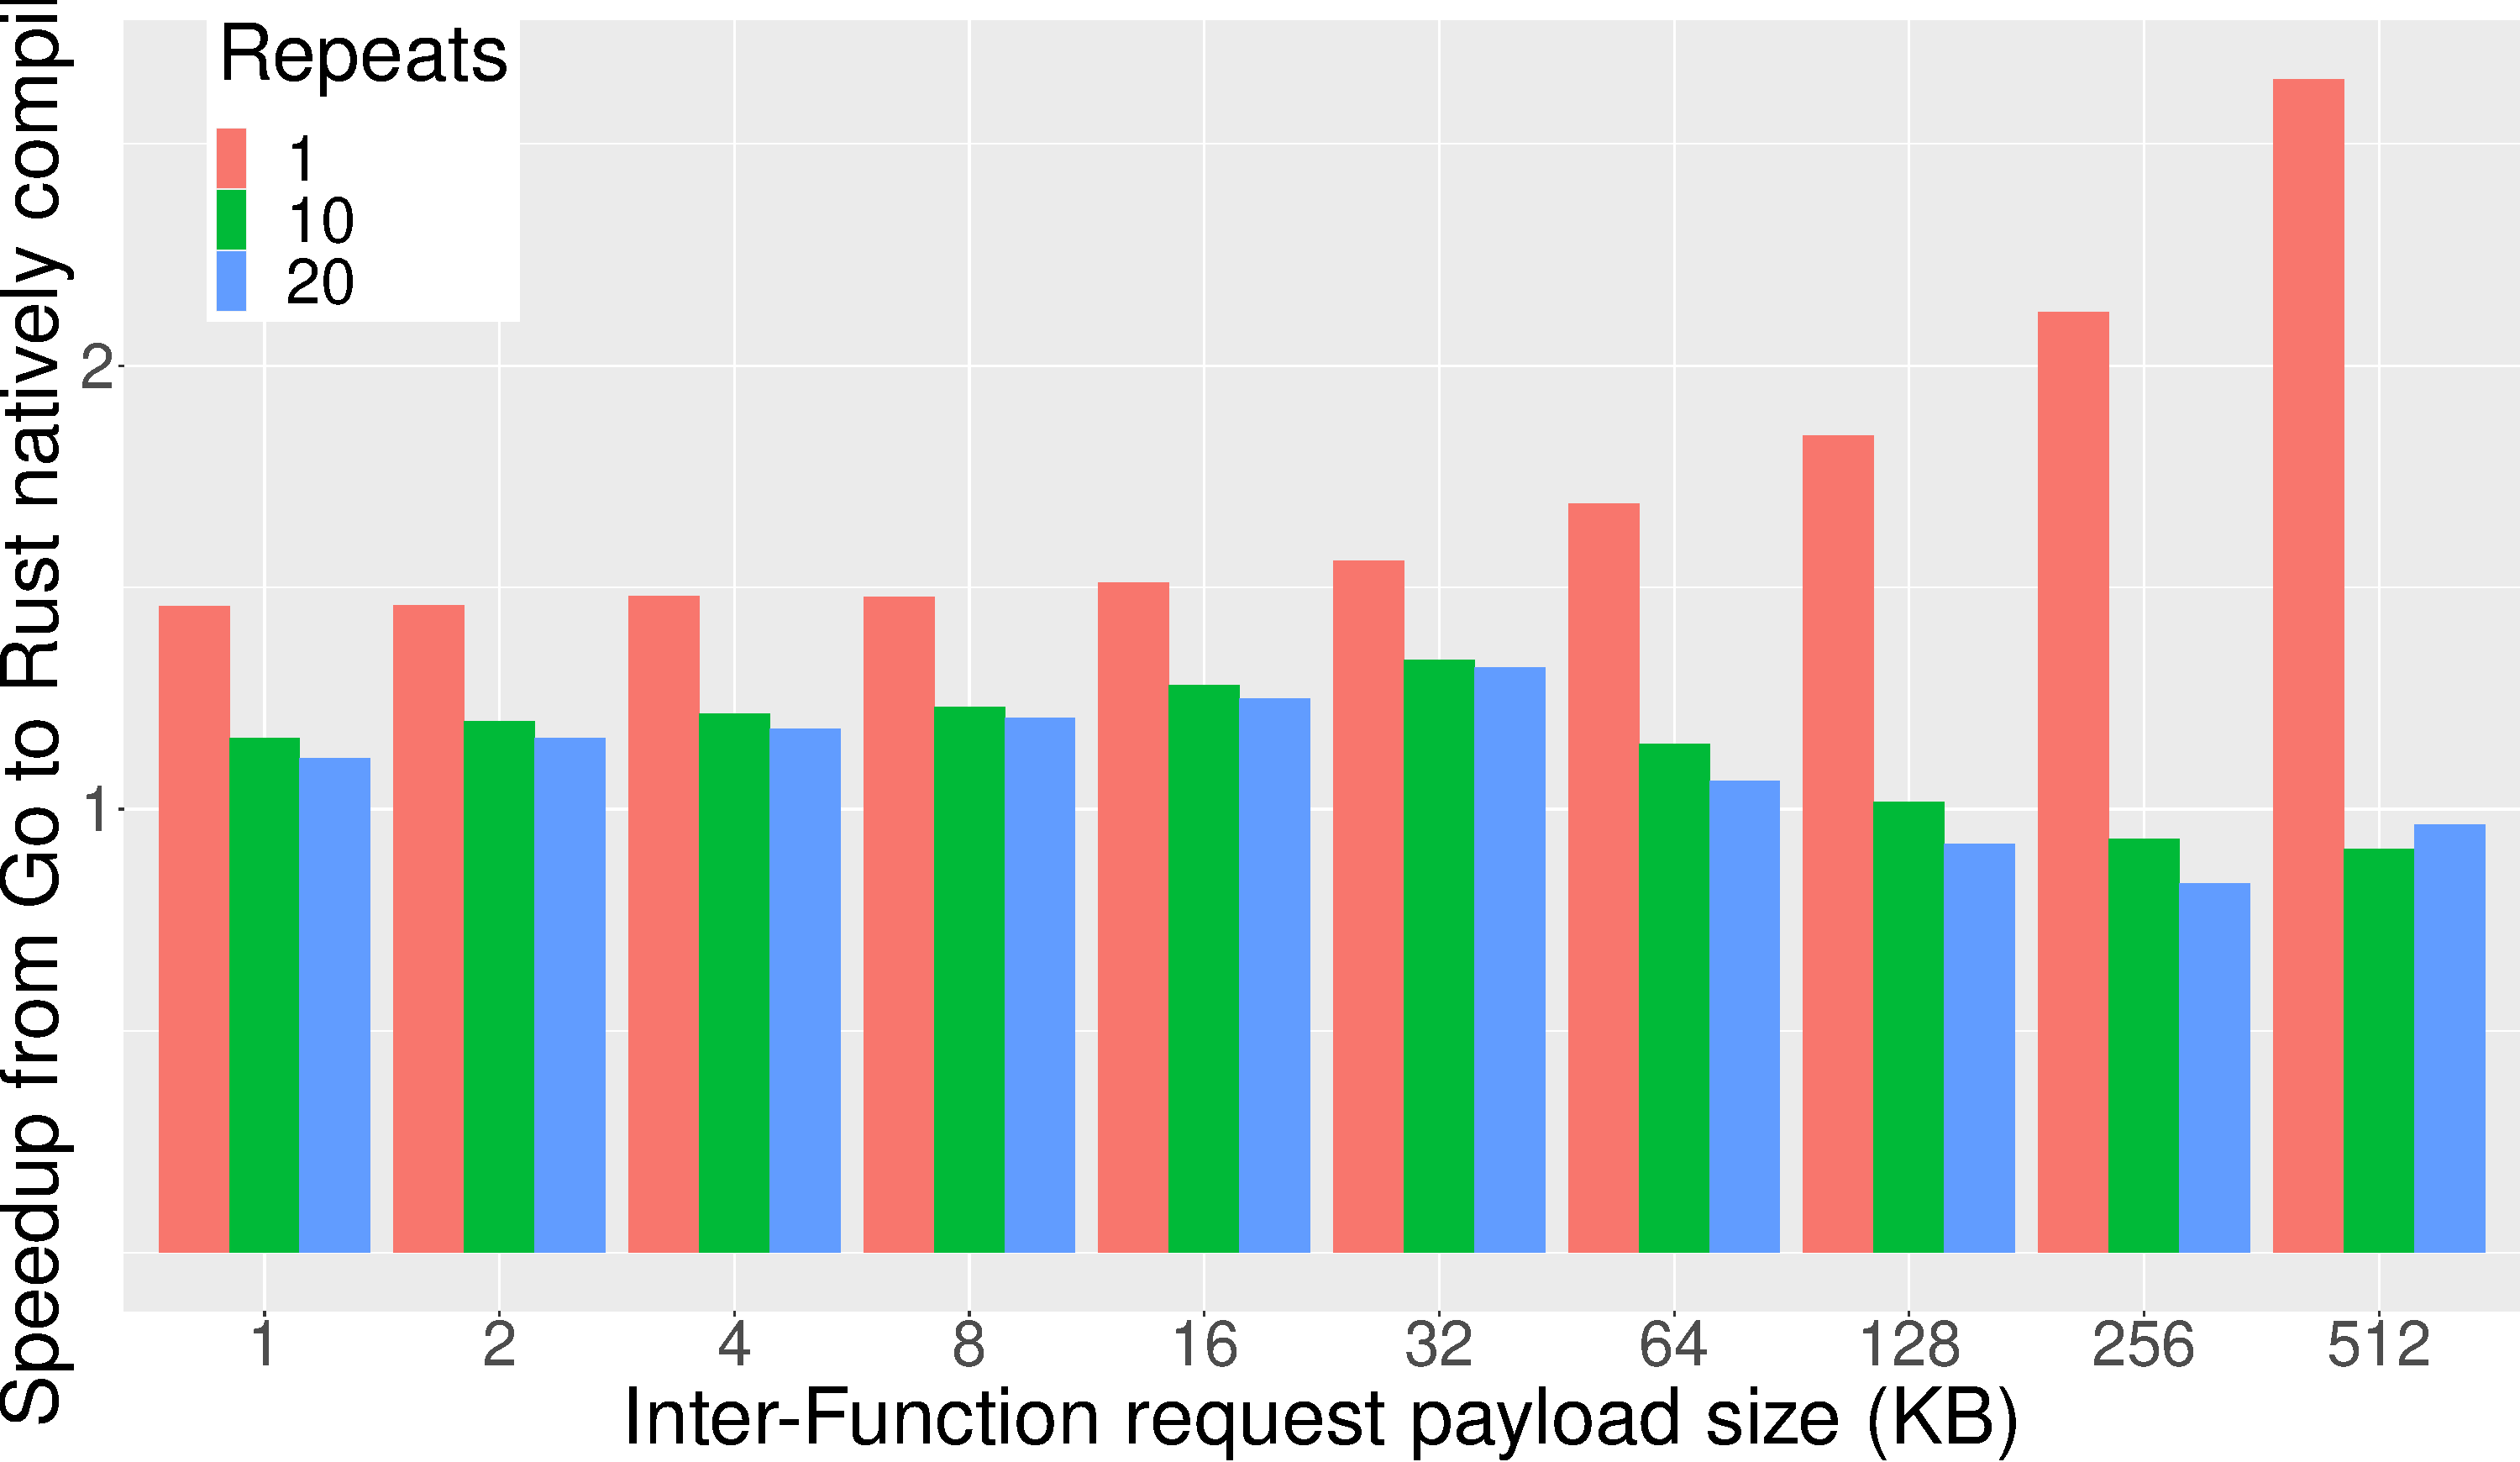
\includegraphics[width=\columnwidth]{figures/rust-go-native}
%   \caption{\label{es:fig:rust-go-native} The speedup achieved when switching from Go to Rust languages executed natively.}
% \end{figure}

% \begin{figure}[ht]
%   \centering
%   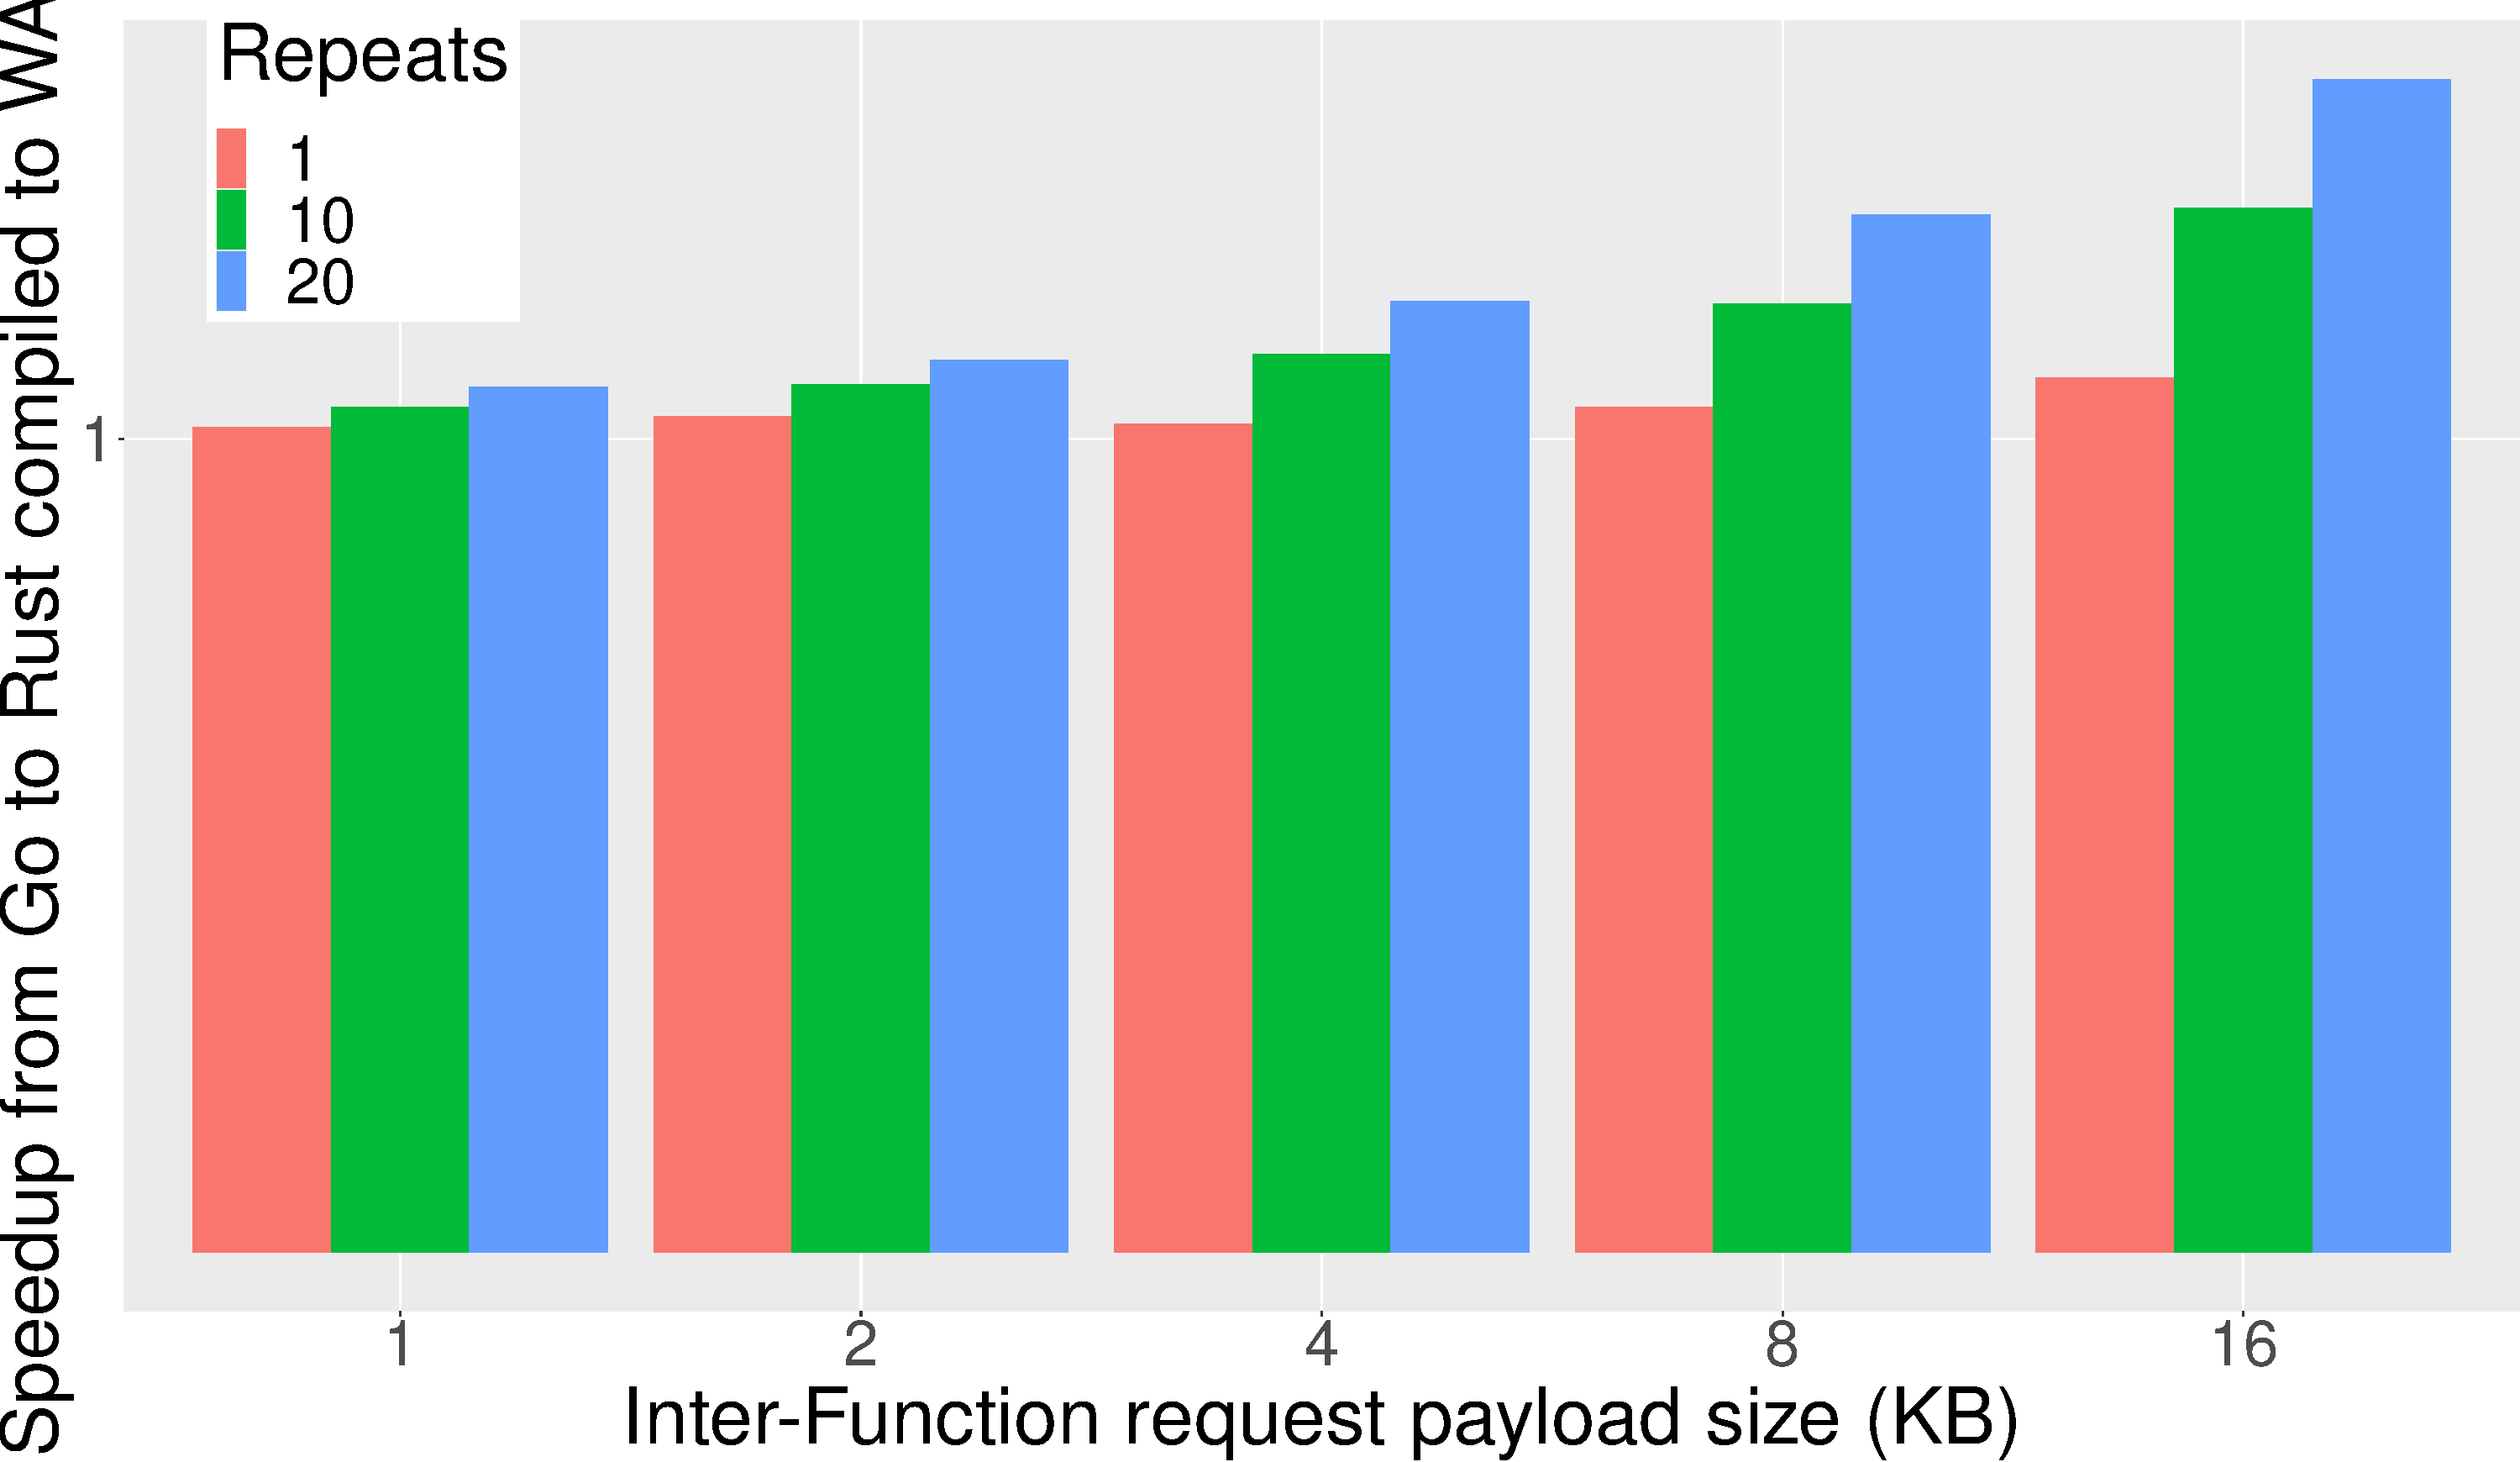
\includegraphics[width=\columnwidth]{figures/rust-go-wasm}
%   \caption{\label{es:fig:rust-go-wasm} The speedup achieved when switching from Go to Rust executed as Wasm.}
% \end{figure}

\begin{figure}
  \centering
  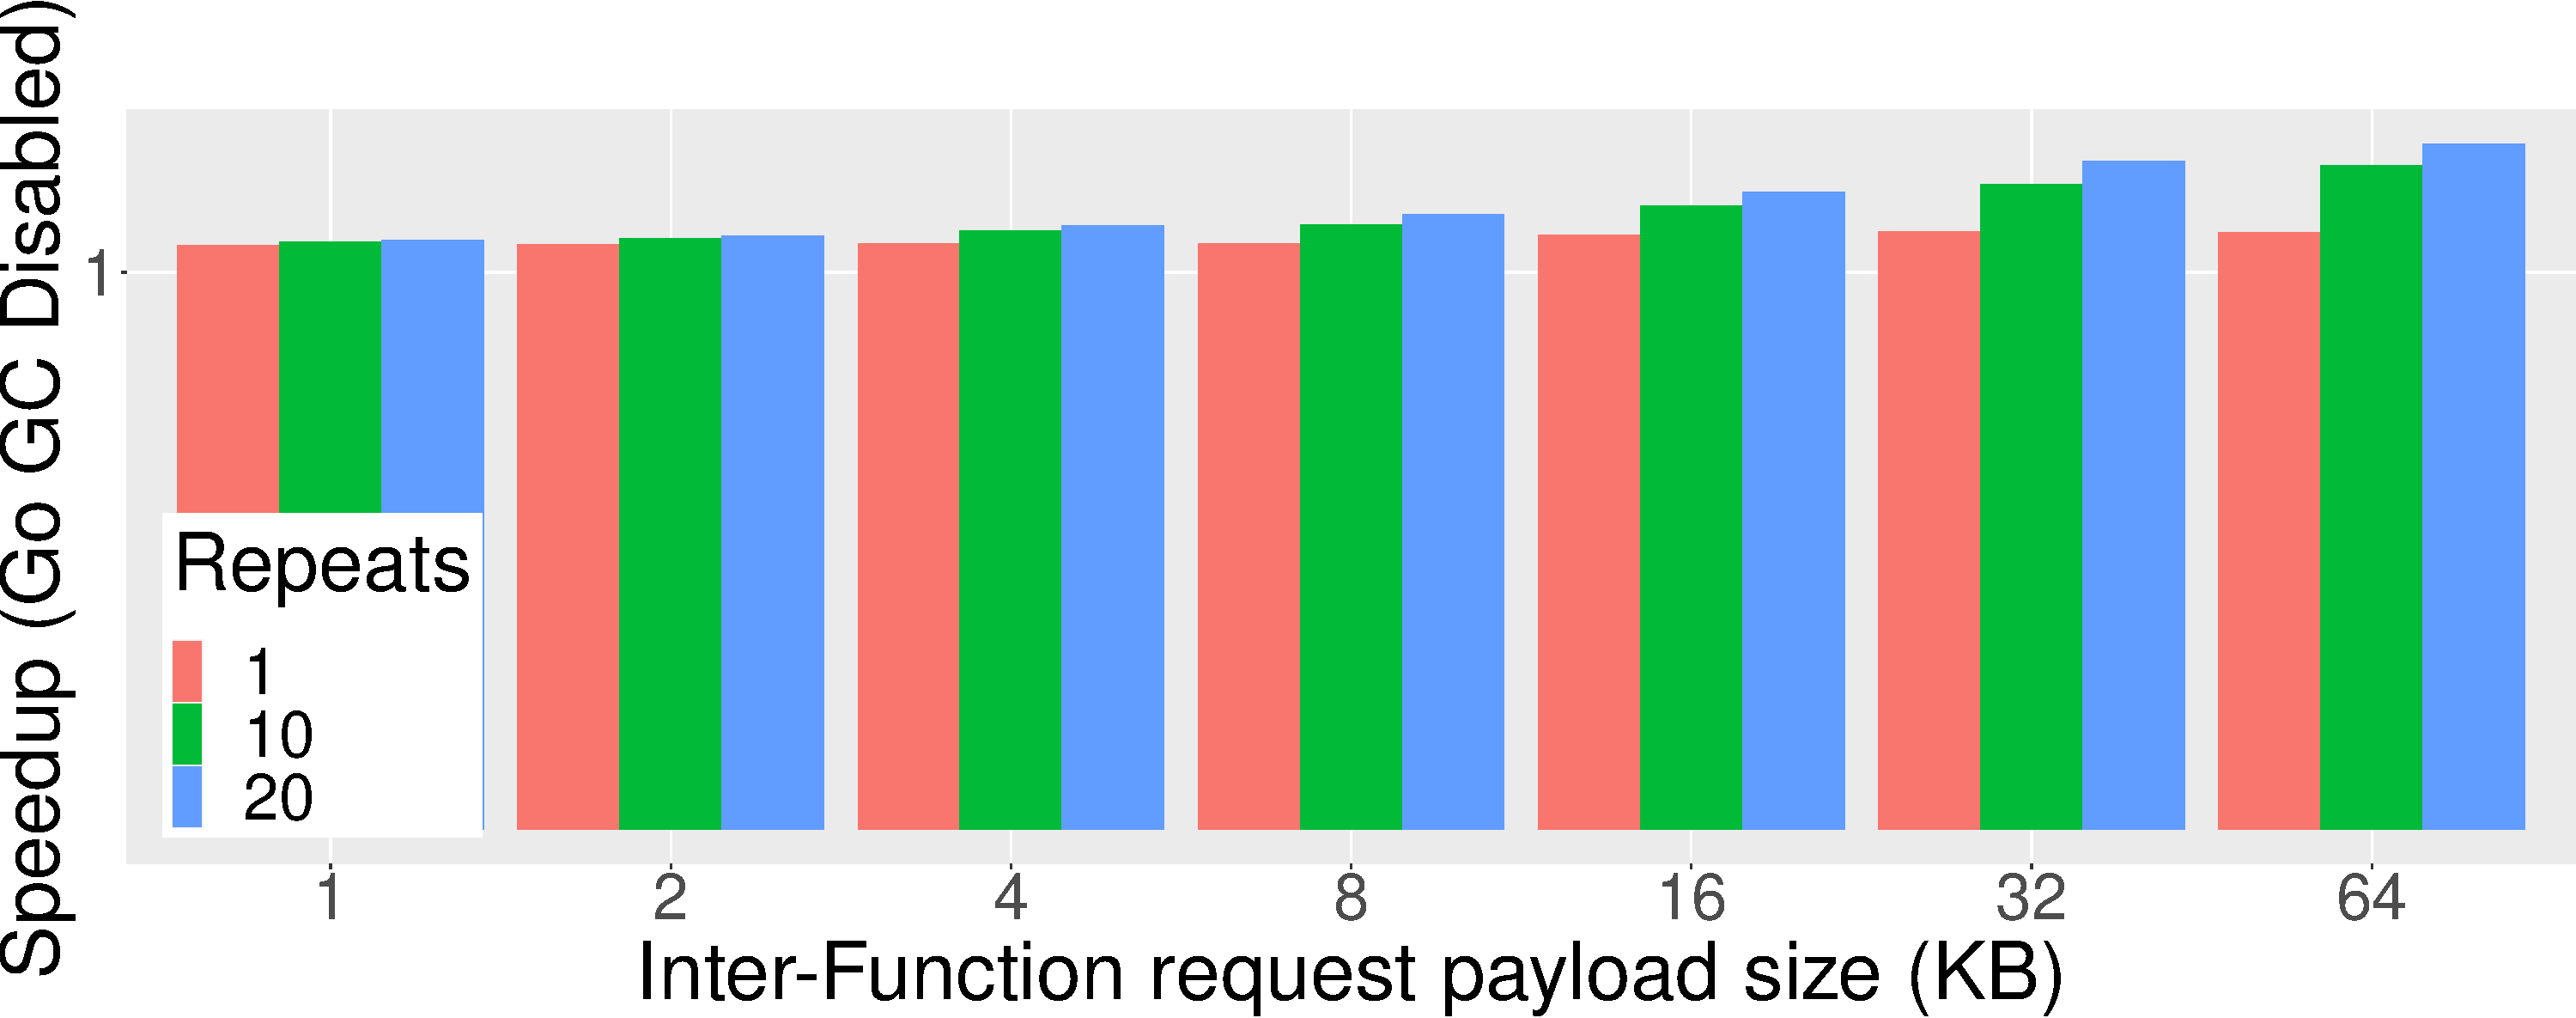
\includegraphics[width=\columnwidth]{figures/go-gc}
  \caption{\label{es:fig:go-gc} The speedup achieved by disabling the Go garbage collector.}
\end{figure}

Recall that we are evaluating the application implemented in Go with GC disabled as described in \Cref{es:sec:methodology}. To ensure that we are not giving the native Go functions an unfair advantage by running them without GC, we examine the impact of disabling GC on the native Go application. The results are presented in \Cref{es:fig:go-gc}. For smaller payload sizes ($\leq$ 8KB) the impact is negligible and for a small advantage of $1.2\times$ to the largest payload size repeated 20 times. From this, we conclude that our decision to disable Go's GC does not skew the results we  presented in \Cref{es:subsec:rtt} and \Cref{es:subsec:intra-app-latency}

\subsection{Transformation Performance}
\label{es:subsec:trans-time}
Applying the CoFaaS transformation to our application written in Go currently takes 1s. As this step comes before compilation, it has only minimal impact on the time needed to compile the application. THe more interesting observation, is that composing CoFaaS components into an application takes just 20ms. This is important because, as stated in \Cref{es:subsec:practice}, compilation can be done ahead of time. Composing CoFaaS functions into a CoFaaS application, however, may be done at deployment time where any additional overheads are much more concerning.

\subsection{Binary Size Implications}
\label{es:subsec:binary-size}

% \begin{figure}[ht]
%   \centering
%   \includegraphics[width=\columnwidth]{example-image-a}
%   \caption{\label{es:fig:binsize} the binary sizes of native and transformed functions}
% \end{figure}

\begin{table}
  \centering
  \caption{\label{es:tab:binsize} The total sizes of containers and binaries needed to run our application.}
  \begin{tabularx}{\columnwidth}{l >{\centering}X >{\centering}X >{\centering}X}
    \toprule
    {\bf Language}  &  {\bf CoFaaS} &  {\bf Native} & {\bf Decrease} \tabularnewline
    \midrule
    {\bf Go}            & 24.5  MB         & 224.0 MB  & $9.1\times$ \tabularnewline
    \midrule
    {\bf Rust}         &  26.3  MB       & 127.1 MB & $4.1\times$ \tabularnewline
    \bottomrule
  \end{tabularx}
\end{table}

Another benefit of CoFaaS is that it reduces the size of the compiled application binaries. While not a primary objective of this work, smaller binaries are beneficial in deployments since they decrease the time and bandwidth needed to store, transfer and bring up an application on a node. \Cref{es:tab:binsize} shows the reductions. The given sizes include the compiled application and any containers and hosts needed to run them. Thus, the sizes given for the native application include the size of the statically compiled function binary and the footprint of the container it is packed in.  The CoFaaS sizes include the Wasm binary containing the CoFaaS optimized and the statically compiled Wasm host runtime needed to run it.  Reducing application image sizes can help reduce the cold-start latency of the application, a much-discussed and central challenge of FaaS deployments (e.g., \cite{du20_catal}). 


% Discuss how the binary sizes are impacted by the CoFaaS transformation. We get some significant savings here especially if we include the size of the containers that FaaS applications usually live in and also the binaries themselves are smaller when compiled to Wasm. This is significant, since fetching and storing binary images uses space and is a component in cold-start latency. 



%%% Local Variables:
%%% mode: latex
%%% TeX-master: "main"
%%% TeX-command-extra-options: "-shell-escape"
%%% End:
